\section{Kiểm tra chất lượng dữ liệu}
\label{sec:3_3}
Phần khảo sát này chỉ sử dụng toàn bộ tệp \texttt{adult.data} gốc, được xem là tập dữ liệu phát triển trước khi chia train và validation ở bước tiếp theo. Tập \texttt{adult.test} được giữ riêng và không dùng để tính các bảng hoặc biểu đồ EDA. Các thống kê là mô tả dữ liệu; bước này chưa quyết định siêu tham số, chưa điền thiếu và chưa loại bản ghi.

Các quy tắc kiểm tra bao gồm tuổi lớn hơn 16, trọng số khảo sát lớn hơn 1, mã học vấn từ 1 đến 16, các khoản vốn không âm và số giờ làm việc từ 1 đến 168 mỗi tuần. Hai điều kiện đầu và điều kiện số giờ dương xuất phát từ mô tả trích xuất dữ liệu; cận 168 là kiểm tra tính hợp lý theo số giờ trong tuần. Miền phân loại được đọc từ \texttt{adult.names}. Dữ liệu thiếu được thống kê riêng, không bị gộp thành giá trị ngoài miền.

Theo các quy tắc đã khai báo, tổng số ô ngoài miền phát hiện được là 0. Kết quả này chỉ phản ánh các kiểm tra trên, không chứng minh dữ liệu hoàn toàn không có lỗi.

\subsection{Giá trị thiếu và giá trị không hợp lệ}
\label{subsec:3_3_1}
Tập phát triển gốc có 2.399 dòng thiếu ít nhất một thuộc tính, chiếm 7,37\%. Giá trị thiếu chỉ xuất hiện ở các cột trong Bảng~\ref{tab:missing-train}. Một dòng có thể thiếu nhiều thuộc tính, nên tổng số ô thiếu không phải số dòng thiếu.

\begin{table}[htbp]
\centering
\small
\caption{Giá trị thiếu trên adult.data gốc}\label{tab:missing-train}
\begin{tabular}{lrr}
\toprule
Thuộc tính & Số ô thiếu & Tỷ lệ (\%) \\
\midrule
occupation & 1.843 & 5,66 \\
workclass & 1.836 & 5,64 \\
native-country & 583 & 1,79 \\
\bottomrule
\end{tabular}
\end{table}

\begin{figure}[htbp]
\centering
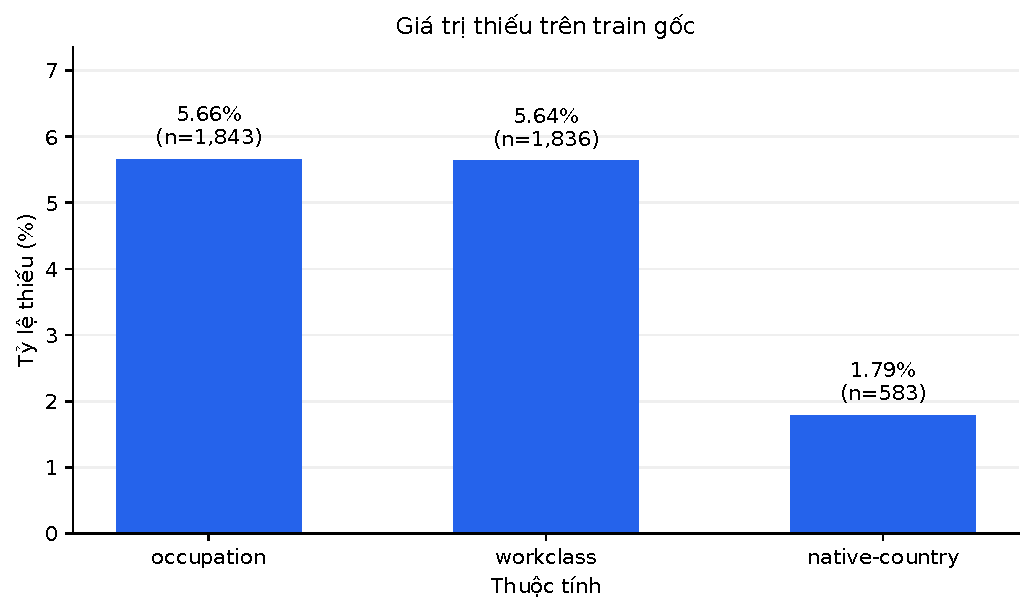
\includegraphics[width=.92\textwidth,height=.72\textheight,keepaspectratio]{Images/chapter_3/3_3/3_3_1/missing_values.pdf}
\caption{Tỷ lệ thiếu tính trên toàn bộ adult.data gốc}
\label{fig:missing-train}
\end{figure}

Các ký hiệu thiếu đã được nhận diện khi đọc dữ liệu. Việc lựa chọn cách điền thiếu sẽ được thực hiện trong pipeline và các giá trị điền được học từ train của từng lần chia, thay vì tính trước trên toàn bộ dữ liệu phát triển.

\subsection{Bản ghi trùng lặp}
\label{subsec:3_3_2}
Hai định nghĩa được khảo sát riêng: trùng toàn bộ 15 cột, gồm cả nhãn, và trùng 14 thuộc tính đầu vào. Số dòng dư là số dòng lặp ngoài lần xuất hiện đầu tiên; số dòng tham gia bao gồm tất cả các thành viên của những nhóm trùng. Giá trị thiếu được xem là cùng một trạng thái khi đối chiếu các hồ sơ.

\begin{table}[htbp]
\centering
\small
\caption{Các dạng trùng lặp trong adult.data gốc}\label{tab:duplicates-train}
\begin{tabular}{lrrr}
\toprule
Định nghĩa & Dòng dư & Dòng tham gia & Số nhóm \\
\midrule
Toàn bộ 15 cột & 24 & 47 & 23 \\
Chỉ 14 đầu vào & 25 & 49 & 24 \\
\bottomrule
\end{tabular}
\end{table}

Có 1 nhóm đầu vào giống nhau nhưng có nhãn khác nhau, gồm 2 dòng. Các trường hợp này được lưu để kiểm tra, chưa bị xóa hoặc gán lại nhãn. Ở bước chia dữ liệu, cần cân nhắc giữ những hồ sơ có cùng đầu vào trong cùng một phía để hạn chế việc các bản sao xuất hiện đồng thời ở train và validation. Phép kiểm tra ở đây chỉ đối chiếu nội bộ dữ liệu phát triển, chưa so sánh với test.

\subsection{Giá trị ngoại lai}
\label{subsec:3_3_3}
Các điểm ngoài khoảng $[Q_1-1{,}5\,IQR,\ Q_3+1{,}5\,IQR]$, với $IQR=Q_3-Q_1$, được đánh dấu để khảo sát. Đây là quy tắc mô tả theo phân vị, không phải kết luận một giá trị nhập sai và không phải quy tắc loại dòng trong pipeline.

\begin{table}[htbp]
\centering
\small
\caption{Các cờ IQR trên sáu thuộc tính số}\label{tab:iqr-train}
\begin{tabular}{lrrrr}
\toprule
Thuộc tính & $Q_1$ & $Q_3$ & Số điểm gắn cờ & Tỷ lệ (\%) \\
\midrule
age & 28,0 & 48,0 & 143 & 0,44 \\
fnlwgt & 117827,0 & 237051,0 & 992 & 3,05 \\
education-num & 9,0 & 12,0 & 1.198 & 3,68 \\
capital-gain & 0,0 & 0,0 & 2.712 & 8,33 \\
capital-loss & 0,0 & 0,0 & 1.519 & 4,67 \\
hours-per-week & 40,0 & 45,0 & 9.008 & 27,66 \\
\bottomrule
\end{tabular}
\end{table}

Đặc biệt, các biến khoản vốn có nhiều giá trị bằng 0. Khi cả hai tứ phân vị bằng 0, IQR cũng bằng 0 và mọi giá trị dương sẽ nằm ngoài hàng rào trên. Vì vậy, không dùng riêng tiêu chuẩn này để loại những hồ sơ có khoản vốn dương.

\begin{figure}[htbp]
\centering
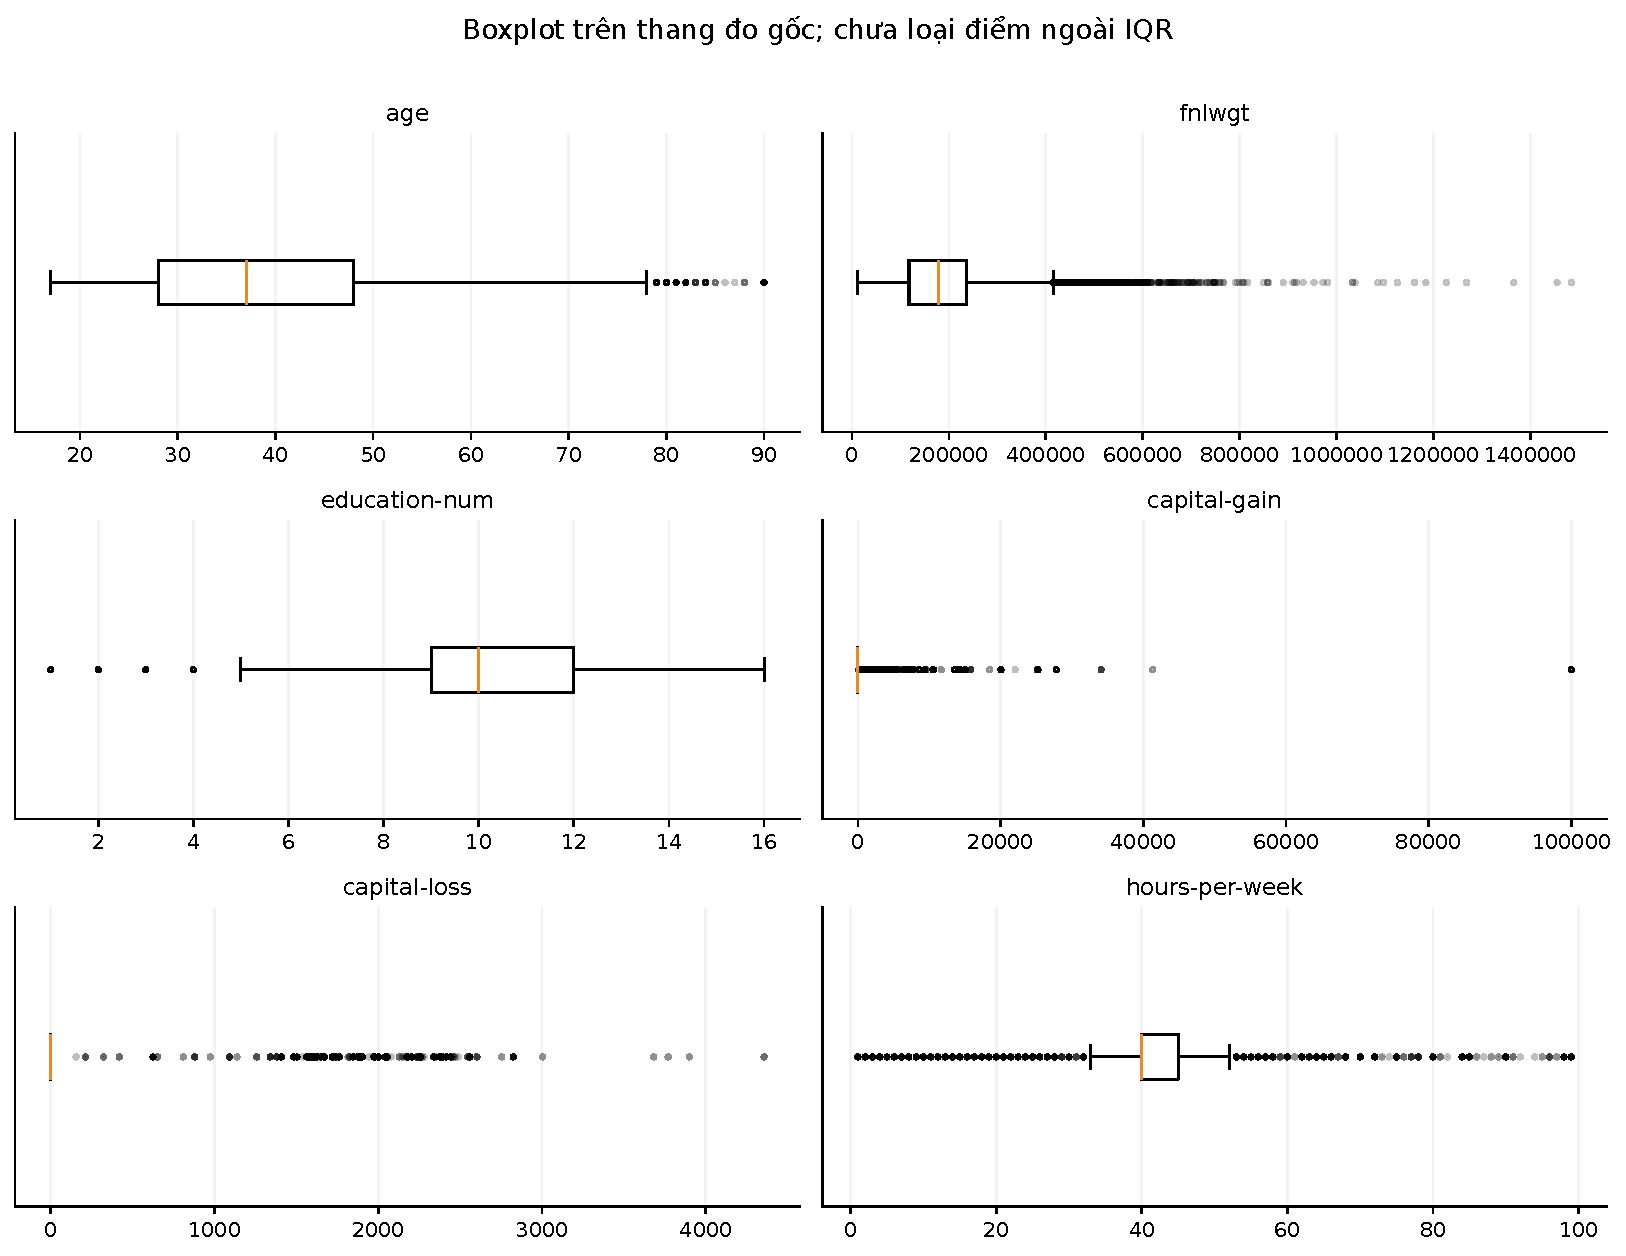
\includegraphics[width=.92\textwidth,height=.72\textheight,keepaspectratio]{Images/chapter_3/3_3/3_3_3/numeric_boxplots.pdf}
\caption{Boxplot riêng cho từng thuộc tính số trên thang đo gốc}
\label{fig:numeric-boxplots}
\end{figure}

